\documentclass[conference]{IEEEtran}
\IEEEoverridecommandlockouts

\usepackage{cite}
\usepackage{hyperref}
\usepackage{graphicx}
\usepackage{textcomp}
\usepackage{xcolor}
\usepackage{float}

\def\BibTeX
{
    {
        \rm B\kern-.05em{\sc i\kern-.025em b}\kern-.08em
        T\kern-.1667em\lower.7ex\hbox{E}\kern-.125emX
    }
}

\hypersetup
{
    colorlinks=true,
    linkcolor=blue,
    filecolor=magenta,      
    urlcolor=cyan,
    pdftitle={Paper V2 - 4squares},
    pdfpagemode=FullScreen,
}

\begin{document}

\title
{
    Servo Comparison\\
    {\footnotesize Botball Standard + Botball Micro vs. Absima S90MH + MEX 85MG}
}

\author
{
    \IEEEauthorblockN{1\textsuperscript{st} Stefan Bleier}
    \IEEEauthorblockA{\textit{Computer Science}\\
    \textit{HTBLuVA}\\
    Wiener Neustadt, Austria\\
    bleier.stefan@student.htlwrn.ac.at}
    \and
    \IEEEauthorblockN{2\textsuperscript{nd} Nico Stolz}
    \IEEEauthorblockA{\textit{Computer Science}\\
    \textit{HTBLuVA}\\
    Wiener Neustadt, Austria\\
    stolz.nico@student.htlwrn.ac.at}
    \and
    \IEEEauthorblockN{3\textsuperscript{rd} Lukas Sanz}
    \IEEEauthorblockA{\textit{Computer Science}\\
    \textit{HTBLuVA}\\
    Wiener Neustadt, Austria\\
    sanz.lukas@student.htlwrn.ac.at}
    \and
    \IEEEauthorblockN{4\textsuperscript{th} Sebastian Lampl}
    \IEEEauthorblockA{\textit{Computer Science}\\
    \textit{HTBLuVA}\\
    Wiener Neustadt, Austria\\
    lampl.sebastian@student.htlwrn.ac.at}
    \and
    \IEEEauthorblockN{5\textsuperscript{th} Raphael Wiedemann}
    \IEEEauthorblockA{\textit{Computer Science}\\
    \textit{HTBLuVA}\\
    Wiener Neustadt, Austria\\
    wiedemann.raphael@student.htlwrn.ac.at}
    \and
    \IEEEauthorblockN{6\textsuperscript{th} Johannes Kosche}
    \IEEEauthorblockA{\textit{Computer Science}\\
    \textit{HTBLuVA}\\
    Wiener Neustadt, Austria\\
    kosche.johannes@student.htlwrn.ac.at}
}

\maketitle

\begin{abstract}
The paper conducts a comparative analysis of botball servos and alternative models to increase design flexibility for OPEN tournament participants and facilitate the servo selection process. The study provides a detailed evaluation of the servos and provides insights that are crucial for informed decision making in hardware selection.
\end{abstract}

\section{Introduction}
This paper provides a comparative evaluation of servos used in botball competitions with comparable models, aiming to establish their performance characteristics. The study assists OPEN-tournament participants in selecting servos that best suit their design needs and implementation requirements. It examines the Absima S90MH and the MEX 85MG servos against their standard and micro botball counterparts across key metrics such as price, size, weight, and speed. The analysis incorporates data from experiments conducted by the authors as well as information from external sources.

\section{Literature Review}
% TODO: Research

\section{Experiments}
\subsection{Price}
Price is often an important factor when choosing servos. It can change depending on where it is purchased, but it is important that all models are similarly priced. If you look closely at the prices, it's clear that the Absima S90MH is more expensive than the standard botball servo. A comparison of the micro botball servo with the MEX 85MG shows a similar situation, but the price difference is smaller. When selecting a servo, one should carefully consider both the cost and the benefits it will bring to the design and operation of the robot.

\begin{figure}[H]
\centering
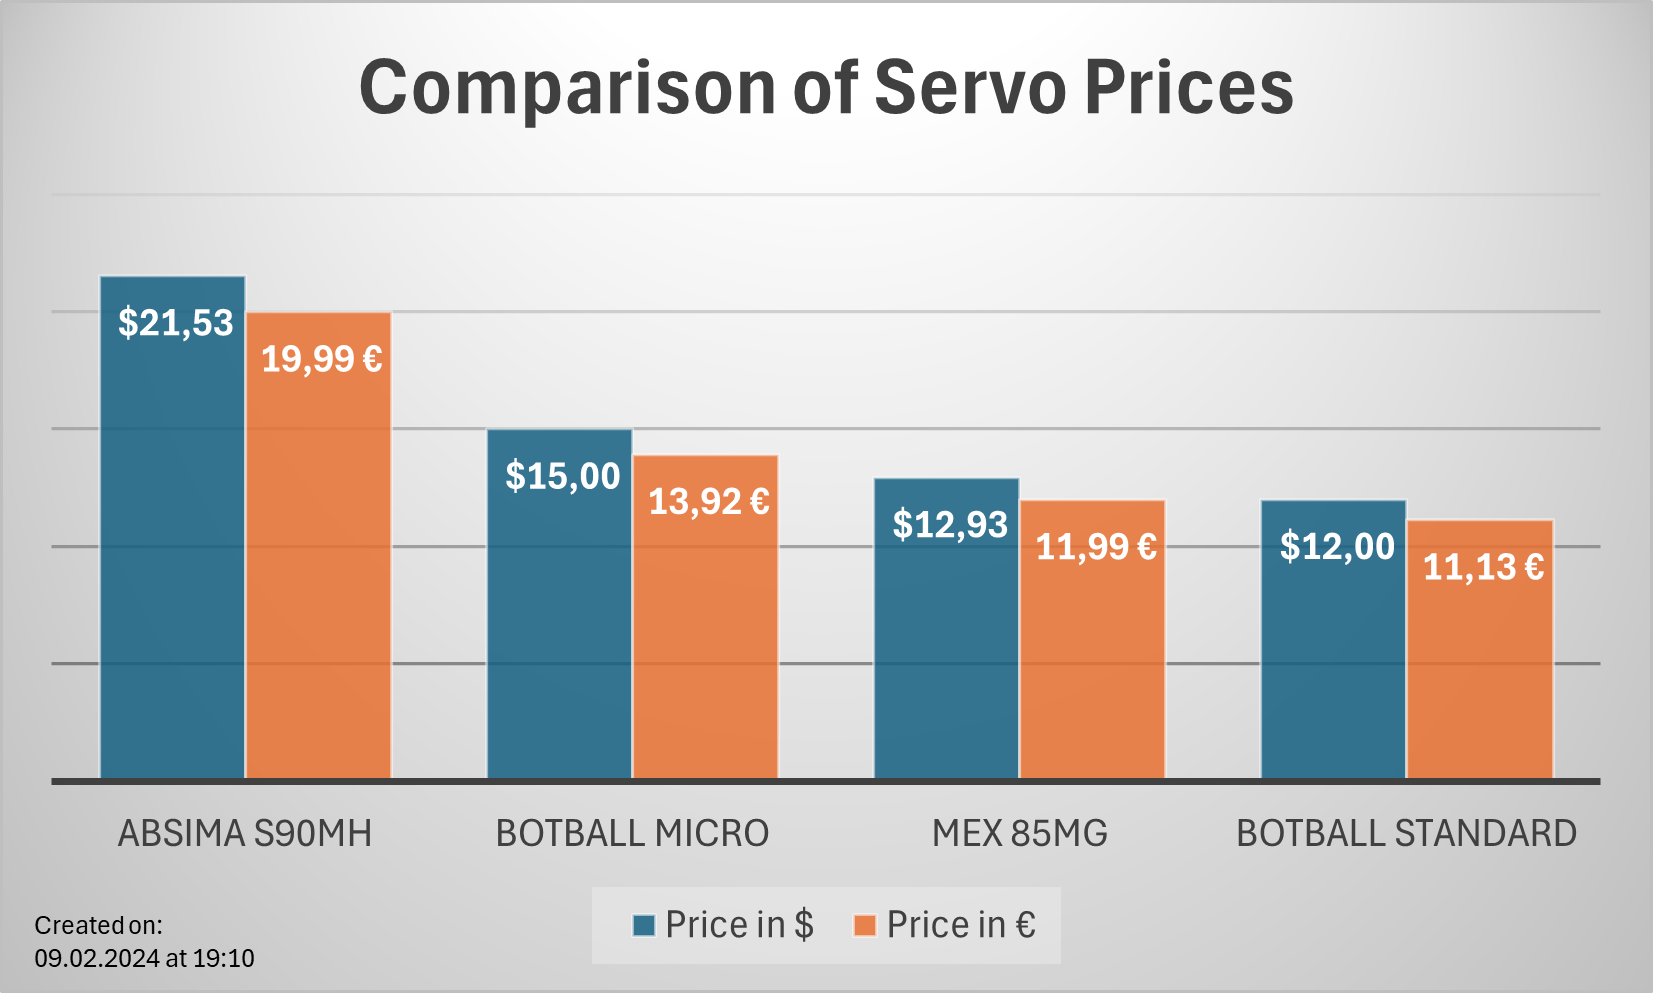
\includegraphics[width=\linewidth]{price_comparison_chart.png}
\caption{Comparison of servo prices in euros and dollars.}
\label{fig:price_comparison}
\end{figure}

The pricing data for this analysis were sourced directly from the official Botball store\textsuperscript{\cite{b1, b2}} and invoice for the comparative models.

\subsection{Size}
Servo dimensions are a pivotal aspect of robot design, especially when dealing with limited space or the need to fit into specific compartments. A servo that is too large can complicate the design process, while a smaller one may offer greater flexibility. Selecting the correct size is therefore essential for optimal robot functionality.

\begin{figure}[H]
\centering
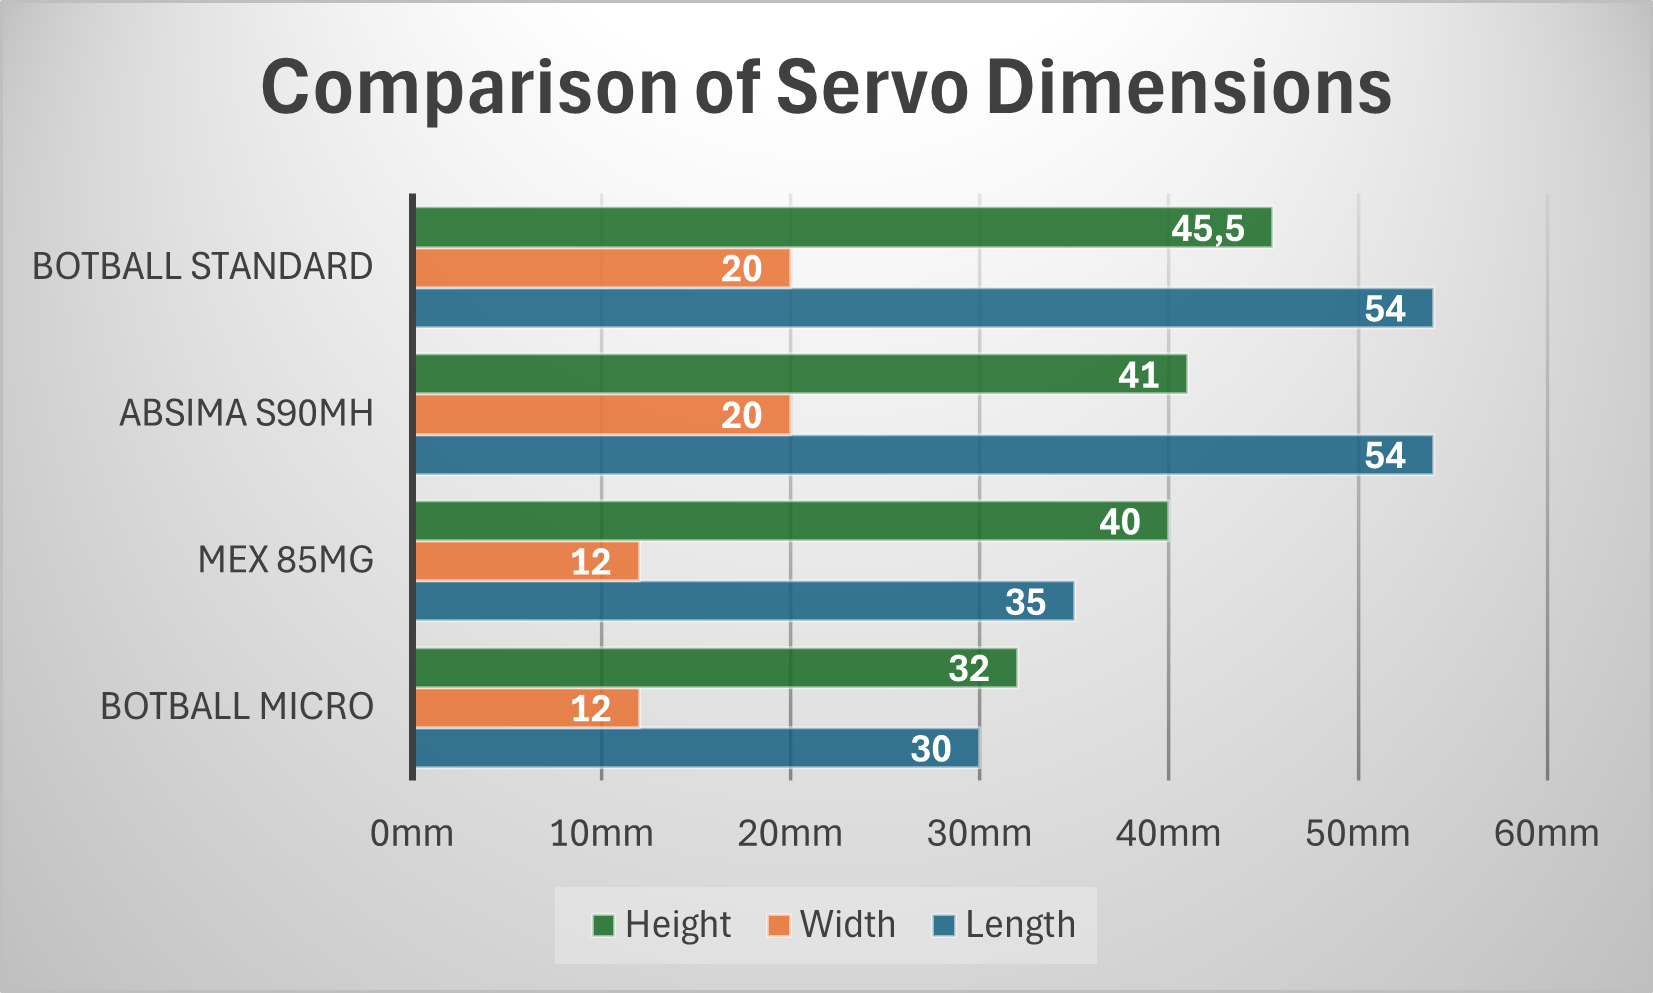
\includegraphics[width=\linewidth]{dimension_comparison_chart.png}
\caption{Comparison of servo dimensions in mm.}
\label{fig:dimension_comparison}
\end{figure}

These measurements were taken using calipers to ensure precision, allowing for an accurate assessment of each servo's size. The data reveals that the standard botball servo has larger overall dimensions compared to the Absima S90MH, whereas the micro botball servo is more compact than the MEX 85MG. Participants in OPEN-tournaments aiming for a smaller robot build will find the micro botball servo to be the best fit. In contrast, projects requiring more robust servos might benefit from the size of the standard botball model. This detailed size comparison aids designers in making easier decisions to meet the specific spatial requirements of their robotics projects.

\subsection{Weight}
Weight plays an integral role in the design and functionality of robots, affecting everything from stability to agility. The choice between a heavier or lighter servo can significantly influence the overall balance of the robot. In some designs, a heavier servo provides necessary stability, especially when placed at the robot's center of gravity. Conversely, lighter servos may be advantageous for applications that require quick movements or have stringent weight restrictions.

\begin{figure}[H]
\centering
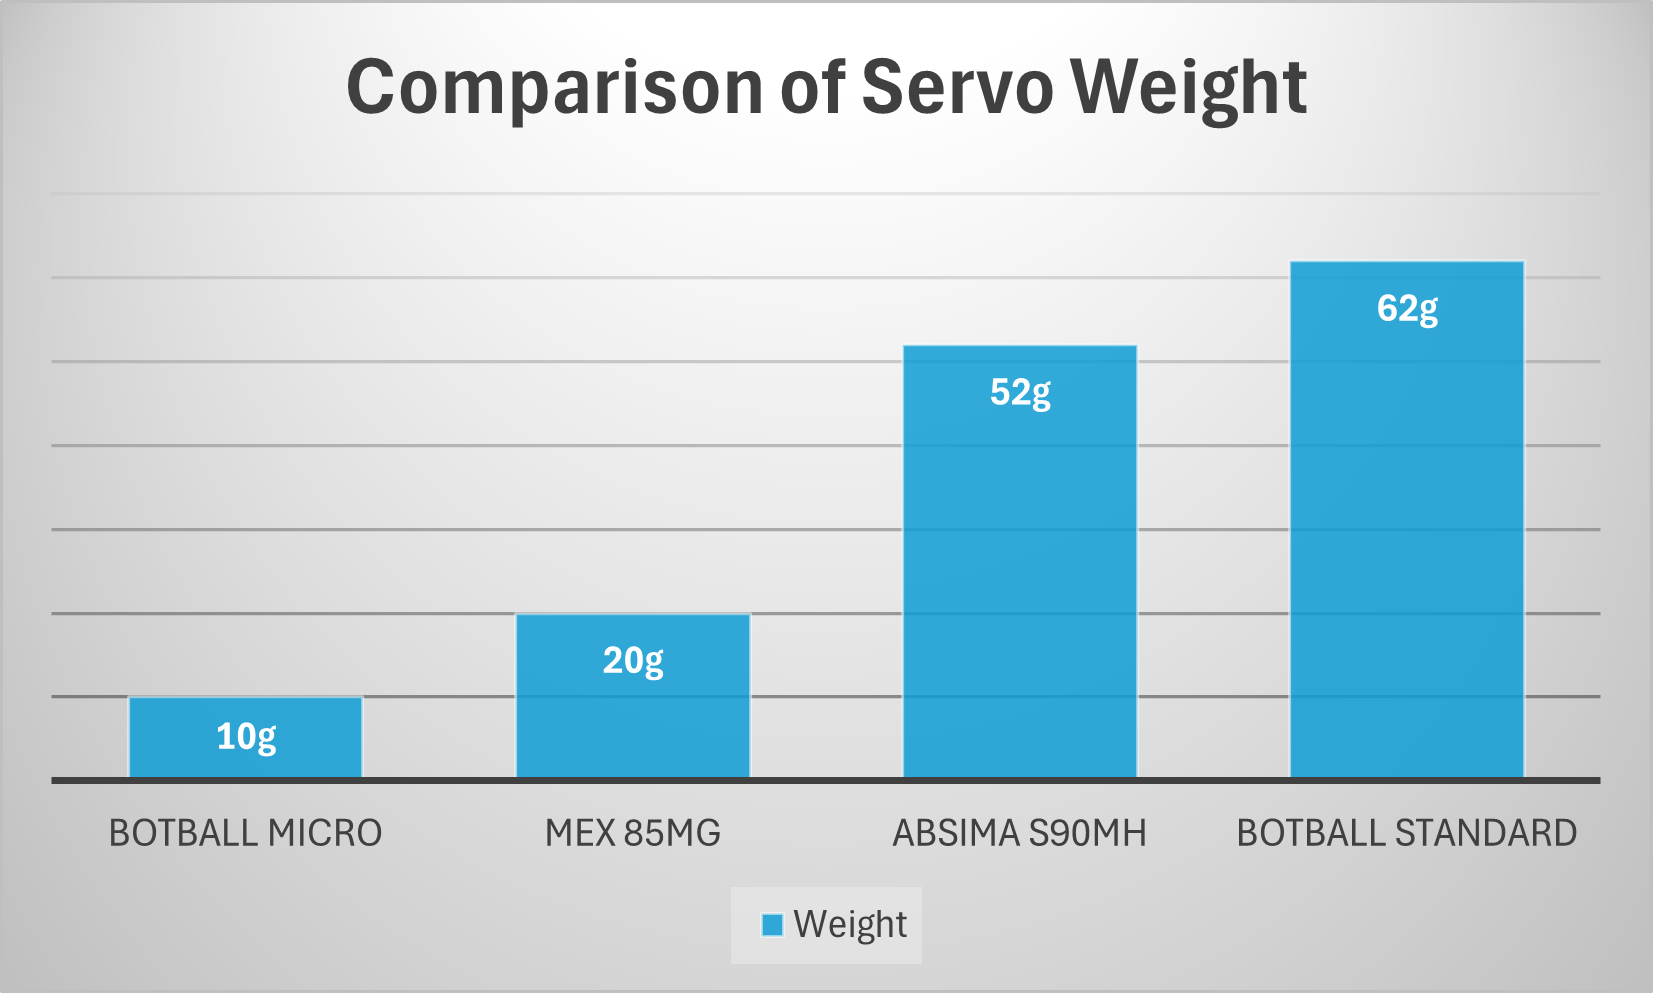
\includegraphics[width=\linewidth]{weight_comparison_chart.png}
\caption{Comparison of servo weight in grams.}
\label{fig:weight_comparison}
\end{figure}

To accurately quantify each servo's weight, precise measurements were taken using a scale capable of measuring to the nearest gram. The data, encompassing both the servo and its cables, offers a direct comparison as depicted in the chart above. As anticipated, there is a correlation between the size and weight of the servos; the micro botball servo is not only smaller in size but also lighter in weight compared to the others. The standard Botball servo, being the largest, also registers as the heaviest. It's important to note that the rotating part of the micro botball servo differs from the others, which may require consideration in its application. Thus, selecting a servo goes beyond mere size and weight—designers must carefully assess how each servo's characteristics align with the specific demands of their project.

\subsection{Speed}
In robotics, especially in competitive environments, the speed at which a servo operates is crucial. A servo must be able to execute movements rapidly to ensure the best performance in competitions. While measuring these quick movements can be complex, this challenge was overcome by capturing high-frame-rate video and analyzing the footage frame by frame, which provides an accurate measure of the servo's speed.

\begin{figure}[H]
\centering
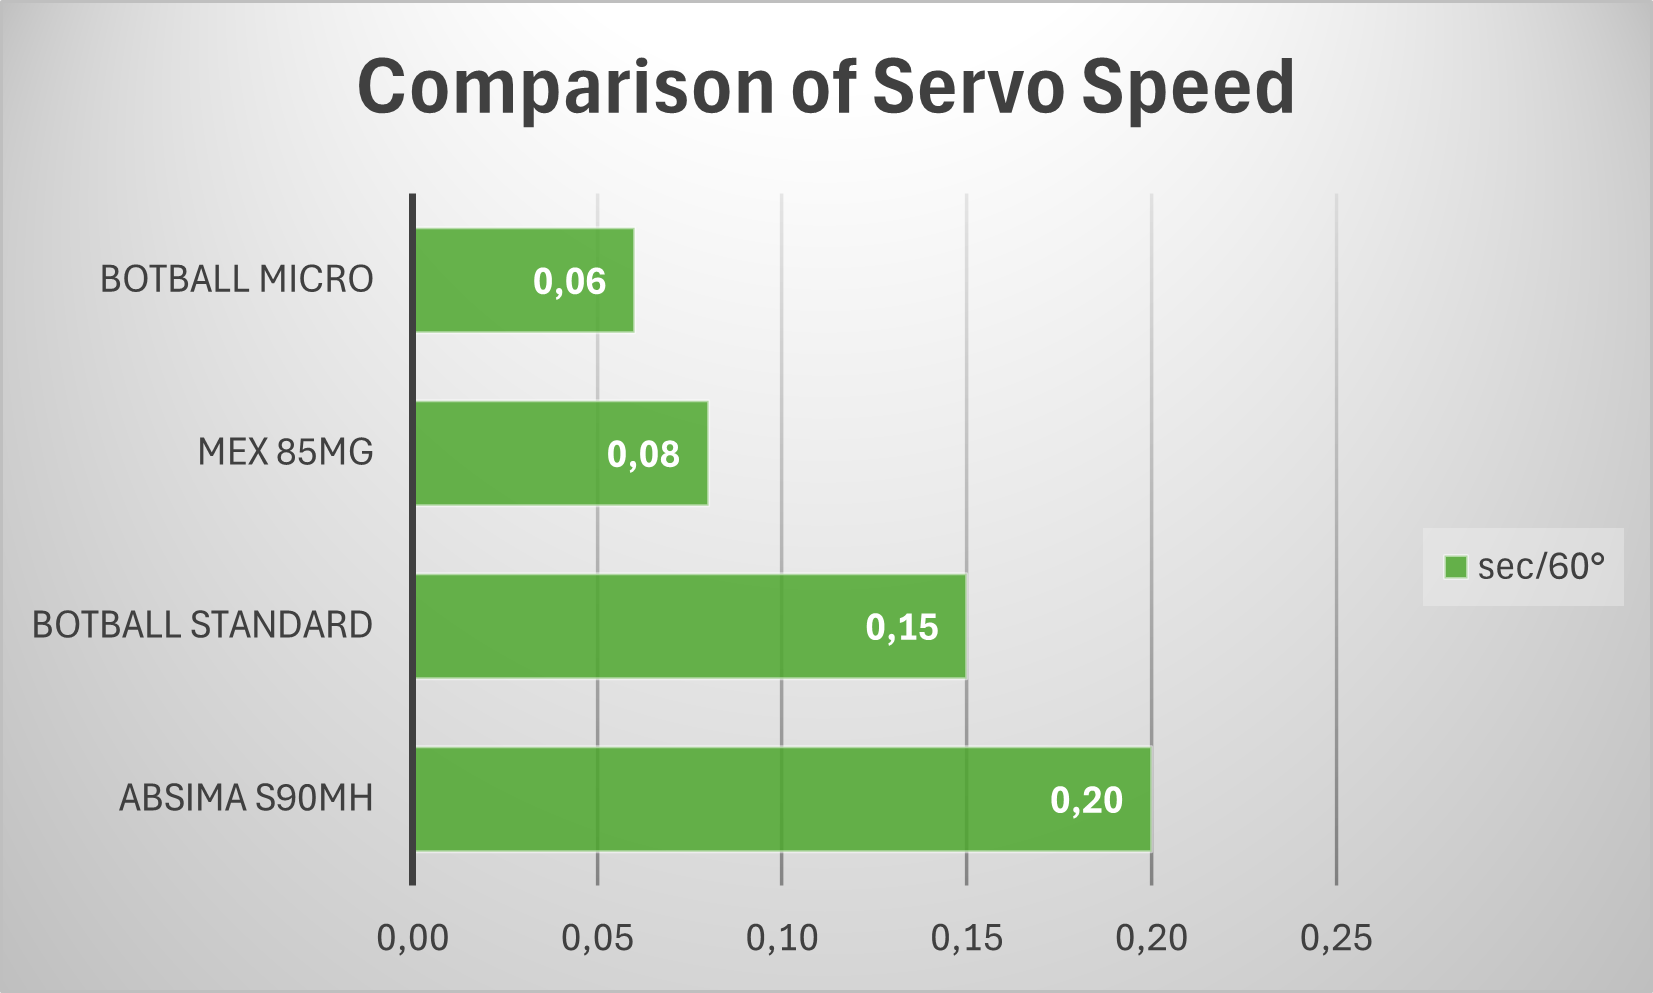
\includegraphics[width=\linewidth]{speed_comparison_chart.png}
\caption{Servo speed comparison, measured in seconds for a 60-degree rotation.}
\label{fig:speed_comparison}
\end{figure}

The analysis of the video data has confirmed that, generally, smaller servos exhibit faster operation speeds than larger ones, making them suitable for applications where rapid response is essential. According to our findings, the Micro Botball servo demonstrates the quickest response, completing a 60-degree turn in just 0.06 seconds. Although the speed differences among the servos are relatively slight, they can be decisive in competitive robotics, highlighting the importance of careful servo selection to meet specific performance criteria.

\section{Conclusion}
The optimal choice of servo is contingent upon its intended application. Data from this study offer valuable insights for tournament participants and hobbyists to determine the most suitable servo for their specific situation. Typically, smaller servos are preferable for tasks requiring agility, while larger ones are favored for applications necessitating greater force. The standard and micro botball servos present viable options for a diverse range of applications.

The Absima S90MH excels in tasks demanding substantial lifting power, surpassing the standard botball servo in capacity, albeit with reduced speed. Its compact size and lower weight make it an attractive alternative, provided the cost is justified. Where budget permits, the Absima S90MH is recommended when the standard botball servo's capacity is insufficient.

Conversely, the micro botball servo stands out for tasks that benefit from high speed and low weight. It outperforms the MEX 85MG in velocity while being marginally larger. For designs prioritizing speed over lifting capability, the micro botball servo is recommended, whereas the MEX 85MG should be considered when a balance between weight and performance is required.

\begin{thebibliography}{00}

\bibitem{b1} Price of the Standard Botball Servo: https://botball-swag.myshopify.com/collections/motos-and-servos/products/standard-servo
\bibitem{b2} Price of the Micro Botball Servo: https://botball-swag.myshopify.com/collections/motos-and-servos/products/micro-servo

\end{thebibliography}

\end{document}